\documentclass{standalone}
\usepackage{tikz}
\usetikzlibrary{arrows.meta}

\begin{document}
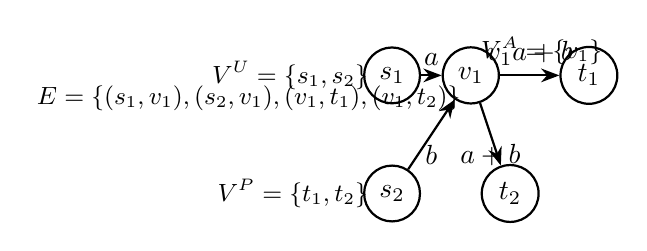
\begin{tikzpicture}[node distance={15mm}, thick, main/.style = {draw, circle}] 
    \node[main] (start1) {$s_1$}; 
    \node[main] (start2) [below of=start1] {$s_2$};
    \node[main] (interm) [right of=start1,xshift=-0.5cm,yshift=0cm] {$v_1$}; 
    \node[main] (end1) [right of=interm] {$t_1$};
    \node[main] (end2) [right of=start2] {$t_2$};
    
    \draw[->,>=Stealth] (start1) -- node[midway, above] {$a$} (interm);
    \draw[->,>=Stealth] (start2) -- node[midway, below] {$b$} (interm);
    \draw[->,>=Stealth] (interm) -- node[midway, above] {$v_1a + b$} (end1);
    \draw[->,>=Stealth] (interm) -- node[midway, below] {$a + b$} (end2);

    % Annotations for the edges
    \node at (start1) [left, xshift=-5pt] {\small{$V^U = \{ s_1, s_2 \}$}};
    \node at (start2) [left, xshift=-5pt] {\small{$V^P = \{ t_1, t_2 \}$}};
    \node at (interm) [above right] {\small{$V^A = \{ v_1 \}$}};
    \node at (interm) [below left] {\small{$E = \{ (s_1, v_1), (s_2, v_1), (v_1, t_1), (v_1, t_2) \}$}};
\end{tikzpicture}
\end{document}